%%%% for public version, toggle \draftfalse in setup2modes.tex
%    (that removes all comments, the blog)

% reducesymm/cgang/2modes.tex    this is master file:    pdflatex 2modes
%     then:    pdflatex def2modes; bibtex def2modes; pdflatex def2modes; pdflatex def2modes

% until 2012-08-20 this was in svn repo siminos/cgang/2modes.tex

\documentclass[aip,cha,
reprint,
secnumarabic,
nofootinbib, tightenlines,
nobibnotes, showkeys, showpacs,
groupedaddress,
%preprint,%
%author-year,%
%author-numerical,%
]{revtex4-1}

\newcommand{\version}{atlas ver. 1.1, Nov 16 2013}
% Burak                     ver. 1.0, Oct  6 2013
% Predrag                   ver. 0.3, Aug  1 2012
% Predrag                   ver. 0.2, Apr 30 2012}
% Predrag from atlas12      ver. 0.1, Apr 25 2012}

        \input setup2modes
        \input ../inputs/def
        \input def2modes

\begin{document}

\title[Low-dimensional cartography]
{Cartography of a 4-dimensional flow with a continuous symmetry:
How to slice it}

\author{Burak Budanur}
\email{budanur3@gatech.edu}
\author{Daniel Borrero-Echeverry}
% \author{Keith M. Carroll} %no response by 2013-08-28
\author{Predrag Cvitanovi\'{c}}
% \author{Bryce Robbins} %no response by 2012-07-26, readded 2013-08-28
\author{Evangelos Siminos}
% \author{Lei Zhang} %no response by 2012-07-26, removed
\affiliation{
 School of Physics and Center for Nonlinear Dynamics,
 Georgia Inst. of Technology,
 Atlanta, GA  30332, USA
}
    \ifdraft
\date{\today}
    \else
\date{1 September 2013}
%\affiliation{
% School of Physics and School of Mathematics,
% Georgia Inst. of Technology,
% Atlanta, GA  30332, USA
% \\\\
% Georgia Tech PHYS 7224 spring 2012 course project
% \\
% \emph{Advisers:
% Predrag Cvitanovi\'{c},
% Daniel Borrero-Echeverry
% and
% Evangelos Siminos}
%}
   \fi


    \begin{abstract}

Danglmayr~\cite{Dang86} and Porter~\&\ Knobloch~\cite{PoKno05} have
introduced a family of 2-Fourier mode \SOn{2}-equivariant ODEs  in order to
study bifurcations of solutions of dynamical systems in presence of
symmetries. A 4-dimensional system of this kind is perhaps the simplest
example of a system with a continuous symmetry that can exhibit chaos, so
we use it to illustrate the role symmetries play in chaotic dynamics. We
show that a continuous symmetry induces drifts in the 4-dimensional state
space dynamics, drifts which obscure the chaotic dynamics. Change of
equations of motions to a locally symmetry-invariant `comoving' frame
does not eliminate these drifts: that is only attained by a
\emph{symmetry reduction} - reformulation of dynamics in a 3-dimensional
symmetry-reduced state space, where every group orbit (set of all points
reached by actions of the group of all symmetries of the equations of
motion) is replaced by a point. Porter~\&\ Knobloch system is a
particularly nice illustration of how this works, as in 3 dimensions we
are able to visualize everything.

We compare three symmetry reduction methods: polar coordinates, invariant
polynomial bases, and the `method of slices'. An invariant polynomial
basis is convenient for determination of all relative equilibria of such
system. Our conclusion, however, is that the most insight is offered by
the method of slices. While in general a number of local slices are
needed to cover a strange attractor~\cite{atlas12}, for the Porter~\&\
Knobloch system there we define a unique slice hyperplane that captures
\emph{all} symmetry-reduced dynamics. A Poincar\'e return map within the
slice hyperplane enables us to reduce the dynamics further, essentially
to a unimodal map, and determine, in principle, all relative periodic
orbits of the system. We can visualize each step of this process without
having to project solutions onto a submanifold since the slice hyperplane
for this system is three dimensional.


[...]
Such a representation gives rise to an \SOn{2}-equivariant dynamical system,
trajectories of which are critically effected by the symmetry related structures
such as \reqva\ and \rpo s; thus, the symmetry reduction holds a crucial role
in understanding the dynamics. Method of slices is a technique for reducing
continuous symmetries where one fixes a particular solution as a template in
the \statesp\ and maps nearby solutions onto the hyperplane that is perpendicular
to the group tangent computed at the template point, by acting on them with
the group action. We demonstrate the method of slices by applying it to
radically simple \SOn{2}-equivariant models where only two Fourier modes are present.
We describe a general two-mode system of order 3, and discuss its representations
in the \SOn{2}-equivariant state space, in the polar coordinates, and
in an invariant polynomial basis, which enables us to determine all \reqva\
of the system. We then focus on two examples with topologically
different chaotic dynamics corresponding to two the different choices of
parameters and apply the method of slices on these systems. We show
that one can determine the symbolic dynamics of
all \rpo s of the system by constructing Poincar\'e
return maps on the slice hyperplane. We can visualise each step of the study
without projecting it onto a sub-manifold since the slice hyperplane, for
this four-dimensional case, is three dimensional.
    \end{abstract}

\pacs{02.20.-a, 05.45.-a, 05.45.Jn, 47.27.ed, 47.52.+j, 83.60.Wc}
\keywords{
symmetry reduction,
equivariant dynamics,
relative equilibria,
relative periodic orbits,
slices,
moving frames
}
\maketitle

%\ifdraft\onecolumngrid % 2012-08-06 temporary \onecolumngrid


    \begin{quotation}
Today, it is possible to  [blah blah].
    \end{quotation}

\section{Introduction}
\label{s:intro}

Over the last decade, new insights into the dynamics of  [blah blah]

Our goals here are two-fold:
    \PC{{\bf[2013-10-07]} Burak's and Daniels outline of Das Artikel is
in \reffig{fig:131007outline}.
}
(i)  Illustrate \mslices\ in the lowest\dmn\ setting possible.
(ii) [blah blah].

As a motivation, consider the chaotic dynamics exhibited by the
small-cell \KS\ system studied in \refref{lanCvit07}. Examination of
typical long-time simulations shows that the spatio-temporal chaos arises
from visits to two kinds of unstable patterns, a `central wobble' region
$S_C$, and a symmetric pair of right/left `drifts' $\{S_L,S_R\}$. In
\statesp\ projections orbits stay in one neighborhood for a while, then
hop to another neighborhood, as illustrated in \reffig{f:antlong}. The
strange attractor that they explore is curved and folded in such a way
that a single local linear chart cannot cover the whole attractor,
several charts are needed, as illustrated by \reffig{fig:2ModeAtlas}\,(d).

The \statesp s of \KS\ and fluid-dynamical flows are high\dmn\ and
difficult to visualize, so here we shall illustrate the key ideas by a
much simpler example, the $\SOn{2}$-equivariant  \twoMode\ system.

%%%%%%%%%%%%%%%%%%%%%%%%%%%%%%%%%%%%%%%%%%%%%%%%%%%%%%%%%%%%
\begin{figure} %[tbp] %[h]
    \centering
% 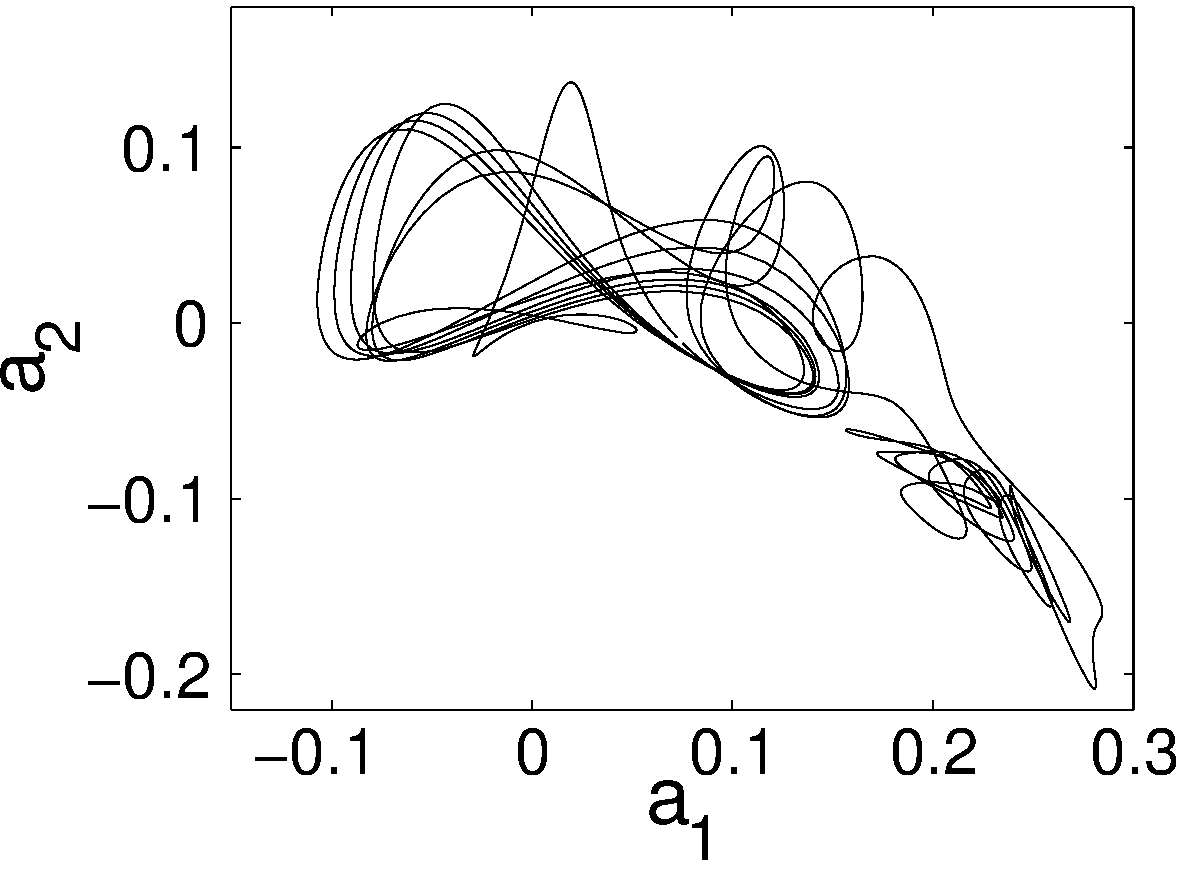
\includegraphics[width=0.40\textwidth]{kslong12}
\caption[]{
A long \KS\ \po\ of period $\period{}=355.34$ that connects
neighborhoods called `$S_C$' and `$S_R$',
(c) $[a_1,a_2]$  projection on the first two spatial Fourier modes
(from \refref{lanCvit07}).
      }
\label{f:antlong}
\end{figure}
%%%%%%%%%%%%%%%%%%%%%%%%%%%%%%%%%%%%%%%%%%%%%%%%%%%%%%%%%%%%%%

%%%%%%%%%%%%%%%%%%%%%%%%%%%%%%%%%%%%%%%%%%%%%%%%%%%%%%%%%%%%%%%%%%%%%
\begin{figure}
%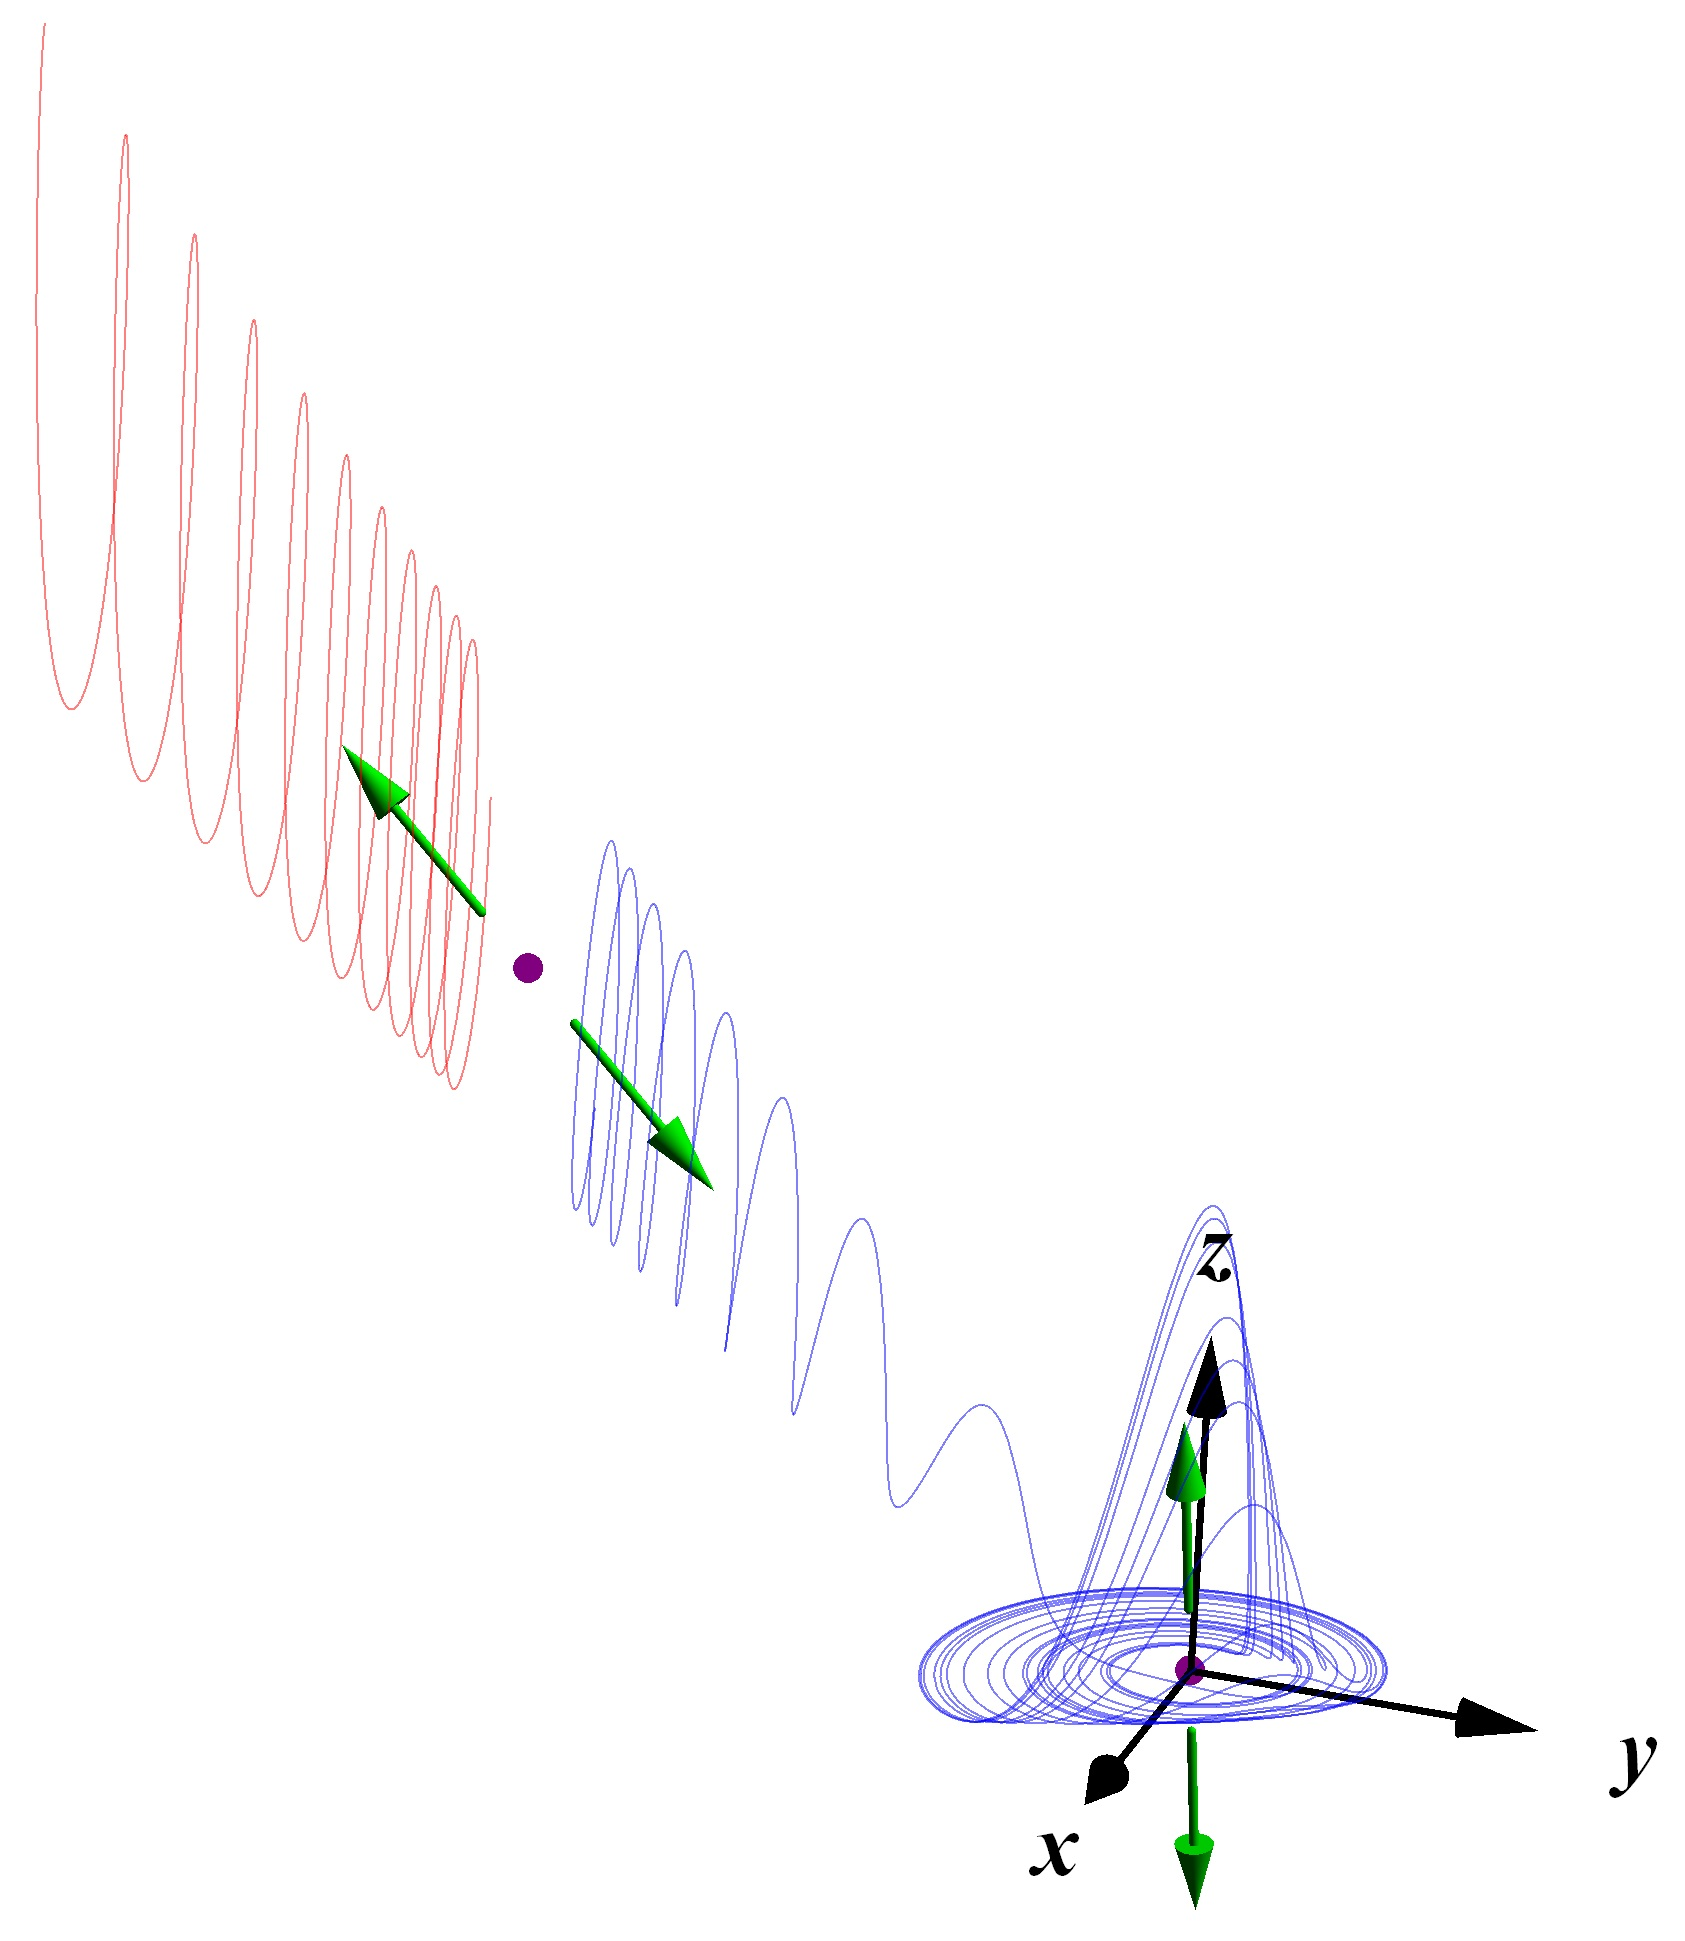
\includegraphics[width=0.28\textwidth]{RoessTrjs2}%{Rossler_Equilibria2}{RoessTrjs}%
 \begin{center}
 \setlength{\unitlength}{0.20\textwidth}
(a)
%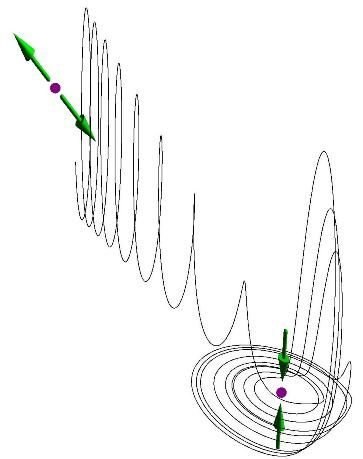
\includegraphics[width=\unitlength,clip=true]{RoessTrajLbld2}
(b)
%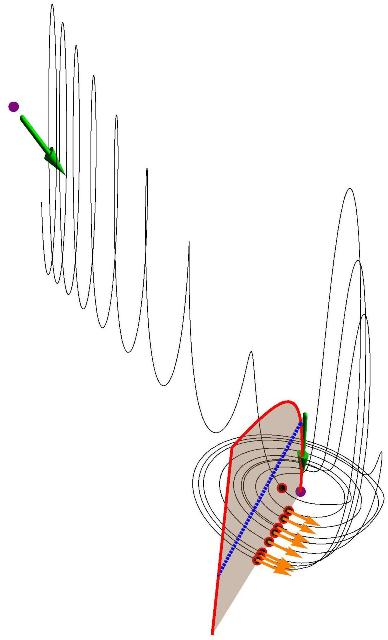
\includegraphics[width=\unitlength,clip=true]{RoessNeareqLbld2}
\\
(c)
%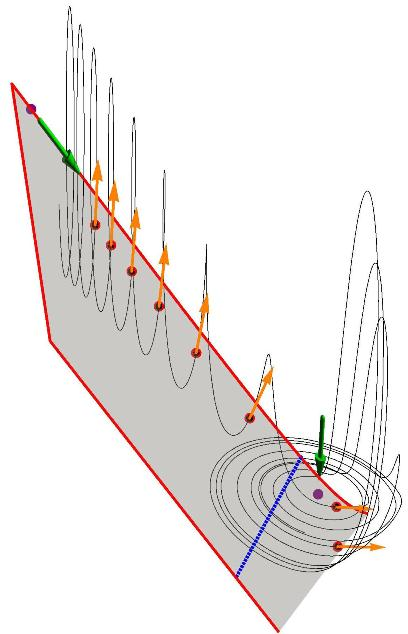
\includegraphics[width=\unitlength,clip=true]{RoessFareqLbld2}
(d)
%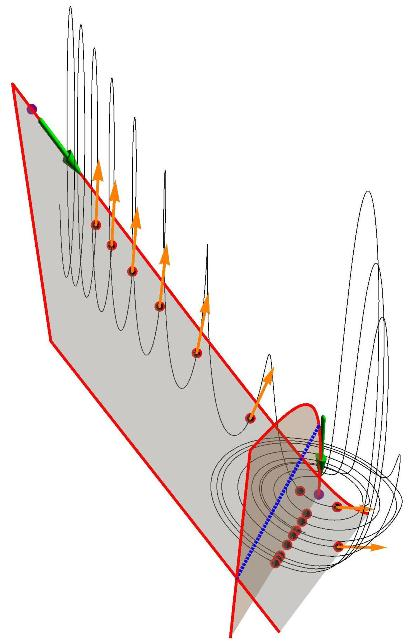
\includegraphics[width=\unitlength,clip=true]{RoessBotheqLbld2}
 \end{center}
    \caption{
2-chart atlas for \twoMode\ flow.
(a)
(b)
(c)
(d)
    }
\label{fig:2modeSects}
\end{figure}
%%%%%%%%%%%%%%%%%%%%%%%%%%%%%%%%%%%%%%%%%%%%%%%%%%%%%%%%%%%%%%%%%%%%%

 [blah blah]

\section{Continuous Symmetries}
\label{s:symm}

A dynamical system, $\dot{\ssp}=\vel(\ssp)$, is equivariant under a continuous
symmetry transformation
\beq
	\ssp'= \LieEl (\theta) \ssp = \exp\left( \theta \Lg\right)\ssp,
\ee{contSymTrans}
if the equivariance condition \rf{DasBuch}
\beq
  \groupTan(\vel)  - \Mvar(\ssp) \, \groupTan(\ssp) =0
  \,,
\ee{inftmInv}
is satisfied for every point of the \statesp . In equations \refeq{contSymTrans} and \refeq{inftmInv},
$\LieEl (\theta)$ is the Lie group element, $\Lg$ is the Lie algebra generator,
$\Mvar(\ssp)_{ij} = {\pde \vel_i}/{\pde\ssp_j} |_x$  is the \stabmat ,
$ \groupTan(\ssp) = \Lg \ssp $ is the group tangent evaluated at the point $\ssp$ ,
and $ \groupTan(\vel) = \Lg \vel(\ssp) $ is the group tangent for the velocity
vector evaluated at \ssp .

\subsection{\Reqva\ and \rpo s}
\label{s:relatives}

If the orbit of a point $\ssp_\stagn$ coincides with its group orbit,
namely if one can find a group parameter $\theta (t)$, for every point $\ssp (t)$
on the orbit of $\ssp_\stagn$ such that
\beq
  \ssp (t) = \ssp_\stagn + \int_0^t d\tau \vel(\ssp (\tau)) = \LieEl (\theta (t)) \ssp_\stagn
  \,
\ee{releq}
is satisfied, the $\ssp_\stagn$ is called a \reqv . By expanding both sides of \refeq{releq}
for infinitesimal time, we can get the relation $\vel(\ssp_\stagn) = \dot{\theta}(\ssp_\stagn) \Lg \ssp_\stagn$,
and since this has to hold for every point on the group orbit of $\ssp_\stagn$
we deduce that $\dot{\theta} = c$ is a constant. We now can multiply the equivariance
condition \refeq{inftmInv} evaluated at the \reqv\ by $c$ and write the
\reqv\ condition compactly as
\beq
(\velRel \Lg - \Mvar ) \vel (\ssp_\stagn) =0
\,.
\ee{ReqvMargEig}
The constant group parameter velocity $c$  is called the \phaseVel .

Similar to the \reqv\ condition \refeq{releq}, \rpo\ condition for a \statesp\ point can be written as
\beq
  \ssp (T) = \ssp_\rpprime  + \int_0^T d\tau \vel(\ssp (\tau)) = \LieEl (\theta_\rpprime ) \ssp_\rpprime
  \,,
\ee{relpo}
meaning that the trajectory of $\ssp_\rpprime$ intersects its group orbit at
time $T$. While the trajectory of a \rpo\ traces out the same path shifted
by the group action over and over again, as we shall see in the examples of
\ref{s:twoModeSymRed}, it can be extremely complicated if the continuous
symmetry of the system is not reduced.

\subsection{Symmetry reduction by the \mslices}
\label{s:slice}

Basic idea of the \mslices\ is picking a particular \statesp\ point as a \template\
($\slicep$) and expressing solutions as reduced trajectories ($\sspRed (t)$) on the hyperplane
(\pSRed) that involves the \template\ ($\slicep$) and is perpendicular to the group
tangent evaluated at the \template\ ($\sliceTan{} = \groupTan(\slicep) = \Lg \slicep$),
while keeping record of the group parameter $\theta (t)$, that maps the solution
back to the symmetry equivariant \statesp . This idea is illustrated in \reffig{fig:ReducTraj1}.

%% ReducTraj*.* - read dasbuch/book/FigSrc/inkscape/00ReadMe.txt
\begin{figure}
\begin{center}
 \setlength{\unitlength}{0.40\textwidth}
 %% \unitlength = units used in the Picture Environment
 \begin{picture}(1,0.8361641)%
   \put(0,0){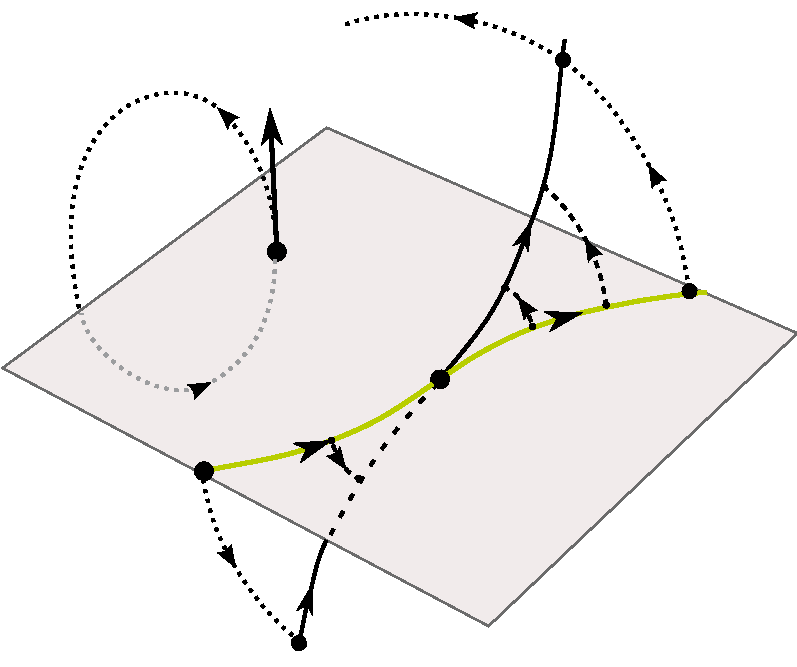
\includegraphics[width=\unitlength]{ReducTraj5.pdf}}%
   \put(0.09054399,0.38282057){\color[rgb]{0,0,0}\rotatebox{-30.34758661}{\makebox(0,0)[lb]{\smash{$\pSRed$}}}}%
   \put(0.57768586,0.29773425){\color[rgb]{0,0,0}\rotatebox{0.0313674}{\makebox(0,0)[lb]{\smash{$\sspRed(0)$}}}}%
   \put(0.59310014,0.69932675){\color[rgb]{0,0,0}\rotatebox{0.03136739}{\makebox(0,0)[lb]{\smash{$\ssp(\tau)$}}}}%
   \put(0.8268425,0.39772328){\color[rgb]{0,0,0}\rotatebox{0.03136739}{\makebox(0,0)[lb]{\smash{$\sspRed(\tau)$}}}}%
   \put(0.81220962,0.66529577){\color[rgb]{0,0,0}\rotatebox{0.03136739}{\makebox(0,0)[lb]{\smash{$\LieEl(\tau)$}}}}%
   \put(0.23150193,0.63610779){\color[rgb]{0,0,0}\rotatebox{0.0313674}{\makebox(0,0)[lb]{\smash{$\LieEl\,\slicep$}}}}%
   \put(0.37740434,0.49597258){\color[rgb]{0,0,0}\rotatebox{0.0313674}{\makebox(0,0)[lb]{\smash{$\slicep$}}}}%
   \put(0.3627714,0.69665188){\color[rgb]{0,0,0}\rotatebox{0.0313674}{\makebox(0,0)[lb]{\smash{$\sliceTan{}$}}}}%
 \end{picture}%
\end{center}
\caption{\label{fig:ReducTraj1}
% (b)
\SlicePlane\ \pSRed\ is a hyperplane % \refeq{PCsect0}
passing through the {\template} point $\slicep$,
and normal to the group tangent $\sliceTan{}$ at $\slicep$.
It intersects all
group orbits (indicated by dotted lines here) in an open
neighborhood of $\slicep$.  The full
\statesp\ trajectory $\ssp(\tau)$ and the \reducedsp\
trajectory $\sspRed(\tau)$ belong to the same group orbit
$\pS_{\ssp(\tau)}$ and are equivalent up to a group rotation
$\LieEl(\gSpace)$ %, defined in   refeq{sspOrbit}
(from \wwwcb{}).
}%
\end{figure}

Reduced trajectories $\sspRed (t)$, can be obtained in two ways. In the first
method, one takes the symmetry equivariant data and looks for the time dependent
group parameter ($\theta (t)$) for which the group operation transforms the
$\ssp (t)$ to $\sspRed (t) = \LieEl(- \theta (t)) \ssp (t)$ that satisfies
the \slice\ condition:
\beq
(\sspRed(t) - \slicep)\cdot \sliceTan{} = 0
\,.
\ee{SliceCond}
This is a post-processing method and is applicable to both numerical and
experimental data, however, as one has to perform a Newton search for
every point in the data set, is computationally heavier than  the second method.
The second method is computing the reduced trajectory $\sspRed (t)$ and the
time dependent group parameter $\theta (t)$ directly by integrating
\bea
\velRed(\sspRed) &=& \vel(\sspRed)
   -\dot{\theta}(\sspRed) \, \groupTan(\sspRed)
\continue
\dot{\theta}(\sspRed) &=& {\braket{\vel(\sspRed)}{\sliceTan{}}}/
               {\braket{\groupTan(\sspRed)}{\sliceTan{}}}
\,.
\label{eq:so2reduced}
\eea
Here, $\velRed$ is the projection of the velocity function on the \slicePlane .
For a detailed derivation of \refeq{eq:so2reduced}, see \refref{DasBuch}.
Note that the time derivative of the group parameter, which appears also
in the reduced velocity function, becomes singular if the dot product $\braket{\groupTan(\sspRed)}{\sliceTan{}}$
is zero. When this happens, the reduced trajectory becomes discontinuous and
no longer useful. The set of points whithin a \slicePlane\ which satisfies
\beq
\braket{\groupTan(\sspRed^*)}{\sliceTan{}} = 0
\,
\ee{ChartBordCond}
is called the \chartBord . In general, \chartBord\ can be avoided by use of
multiple \template s and arranging them in a way that the trajectories do not
intersect the \chartBord , as done in \refref{atlas12}. In the particular
case of the \twoMode\ system that we study in this paper, we can describe
the reduced dynamics using a single \slice\ by picking a \template\ for which
the \chartBord\ is a flow invariant subspace, hence never visited.

If a $d$\dmn\ dynamical flow is $\Group$-equivariant under actions of
an $N$ continuous parameters symmetry group $\Group$, its $d$\dmn\ \statesp\ is foliated
by $N$\dmn\ group orbits, and the symmetry-\reducedsp\
$\pS/\Group$ is $(d\!-\!N)$\dmn.
The simplest continuous symmetry groups are the 1-parameter compact rotation
group $\SOn{2}$ and the 1-parameter noncompact translation group
$T(1)$; here we shall focus on the $\SOn{2}$ case.

In order to construct a representation for $\SOn{2}$ let us take a Fourier
series expansion of a real valued smooth periodic function:
\beq
	u(\phi) = a_0 + \sum\limits_{k=- \infty}^\infty a_k e^{i k \phi} .
\ee{FourierSeries}
We can write the real and imaginary parts of the Fourier coefficients with
$k \geq 1$ in a state vector $(x_1, y_1, x_2, y_2,..., x_m, y_m)$ where
$a_i = x_i + i y_i$ and represent the $\SOn{2}$ group action on this vector
as a block diagonal matrix:
%More explicit form, does not fit in a column:
%\beq
	 %\LieEl (\theta)= \\
					  %\begin{pmatrix}
					  %\cos \theta & \sin \theta & 0               & 0              & \cdots & 0              & 0               \\
					 %-\sin \theta & \cos \theta & 0               & 0              & \cdots & 0              & 0               \\
					  %0             & 0 		   & \cos 2 \theta & \sin 2 \theta & \cdots & 0              & 0               \\
					  %0             & 0            &-\sin 2 \theta & \cos 2 \theta & \cdots & 0              & 0               \\
					  %\vdots       & \vdots      & \vdots         & \vdots        & \ddots & \vdots         & \vdots         \\
					  %0             & 0 		   & 0               & 0              & \cdots & \cos m \theta & \sin m \theta  \\
					  %0             & 0            & 0	             & 0              & \cdots &-\sin m \theta & \cos m \theta
					  %\end{pmatrix}
%\eeq
\beq
	\LieEl(\theta) = \begin{pmatrix}
						R(\theta) & 0 			  & \cdots & 0 \\
						0		   & R(2 \theta) & \cdots & 0 \\
						\vdots	   & \vdots 	  & \ddots & \vdots \\
						0		   & 0	          & \cdots & R (m \theta)
					   \end{pmatrix} ,
\ee{mmodeLieEl}
where,
\beq
	R(n \theta) =	\begin{pmatrix}
					\cos n \theta & \sin n \theta \\
					-\sin n \theta & \cos n \theta
					\end{pmatrix} ,
\ee{rotationmatrix}
are modulated rotation matrices. In this representation, the Lie algebra generator is
\beq
	 \Lg =  \begin{pmatrix}
			 0 & 1 & 0 & 0 & \cdots & 0 & 0 \\
			-1 & 0 & 0 & 0 & \cdots & 0 & 0 \\
			 0 & 0 & 0 & 2 & \cdots & 0 & 0 \\
			 0 & 0 &-2 & 0 & \cdots & 0 & 0 \\
			 \vdots & \vdots & \vdots & \vdots & \ddots & \vdots & \vdots \\
			 0 & 0 & 0 & 0 & \cdots & 0 & m \\
			 0 & 0 & 0 & 0 & \cdots &-m & 0
			 \end{pmatrix} .
\ee{mmodeLg}
Now let us consider the following specific choice of a \slice\ \template\:
\beq
	\slicep = (1, 0, ..., 0) .
\ee{firstmodetemp}
Equation \refeq{SliceCond} restricts the points on the hyperplane defined
by the template point \refeq{slicetemp} to the following form:
\beq
	\sspRed = (\hat{x}_1, 0, \hat{x}_2, \hat{y}_2, ..., \hat{x}_m, \hat{y}_m) .
\ee{slicetemp}
These points satisfy the \chartBord\ condition \refeq{ChartBordCond} only
if $\hat{x}_1 = 0$, in other words, as long as the first mode magnitude is
non zero, there is a corresponding unique point to every group orbit on the
\slicePlane\ defined by \refeq{firstmodetemp}. We pick the \slice\ \template\
\refeq{firstmodetemp} for computational convenience, in general, any first
mode template $\slicep = (x_1, y_1, 0,...,0)$ would do as good since the
first mode has the symmetry of a circle. We also restrict the \slicePlane\
to the half-space where $x_1 > 0$ to have a unique representative point for
each group orbit since otherwise each group orbit pierces the \slicePlane\
twice. These concepts are illustrated in \reffig{fig:BBgorbitsandslice}

\refFig{fig:BBgorbitsandslice} shows a 3D projection of the 4D \statesp\ corresponding
to an $m=2$ truncation of \refeq{FourierSeries}, for which \refeq{mmodeLieEl} and \refeq{mmodeLg}
are $4 \times 4$ matrices. The \slicePlane\ defined by \refeq{firstmodetemp}, three
different group orbits and the group tangents evaluated at their intersections with the \slicePlane\
are visualized in \reffig{fig:BBgorbitsandslice}. One can see as the magnitude of the second mode (the vertical axis)
relative to the first mode increases, the group tangent gets closer to being
parallel to the \slicePlane , however, it still has a non zero perpendicular component. The vertical
axis ($x_2$) in \reffig{fig:BBgorbitsandslice} lies on the \chartBord\ of the
\slicePlane .

In the next section, we will introduce a dynamical system with the four dimensional
\statesp\ geometry of \reffig{fig:BBgorbitsandslice} and analyze its symmetry
reduced dynamics within the \slicePlane\ defined by a \template\ of the form
\refeq{slicetemp}.

\begin{figure}%[H]
\centering
 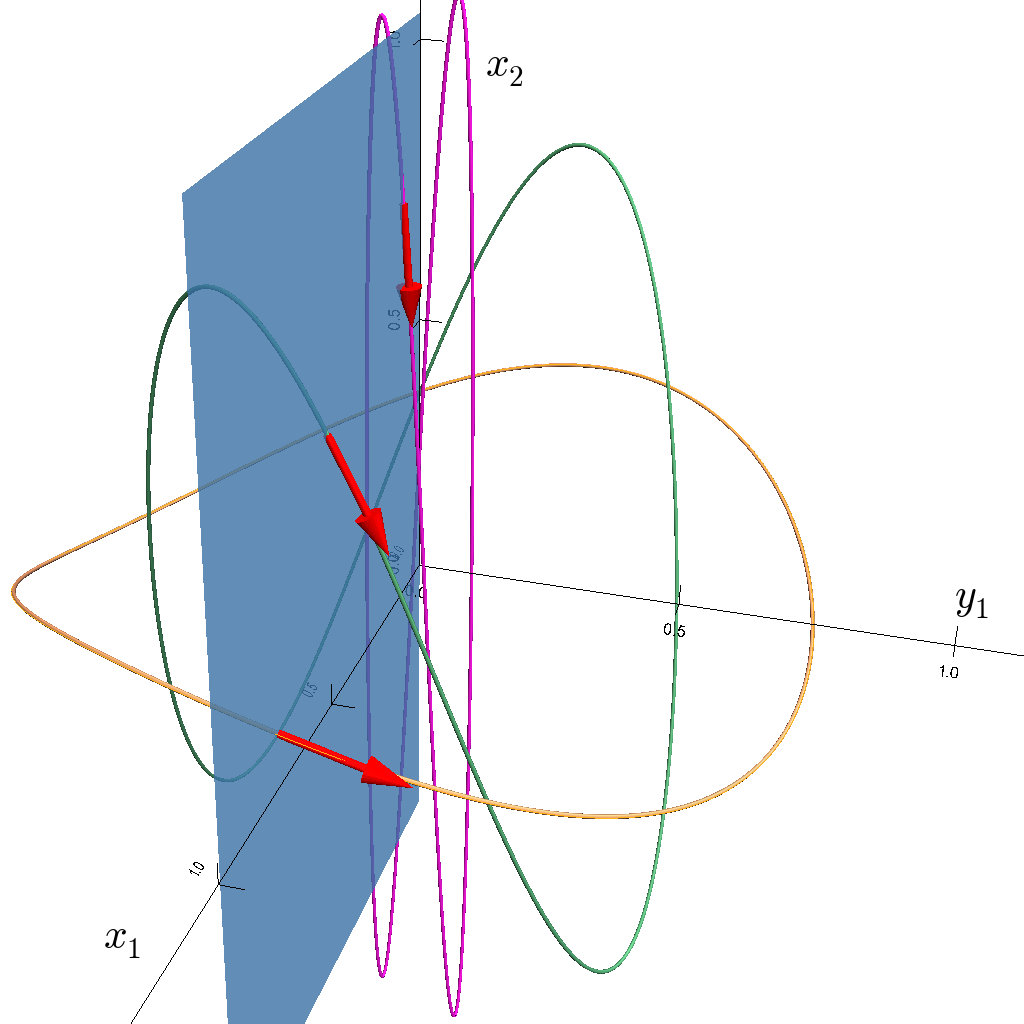
\includegraphics[width=0.45\textwidth]{BBgorbitsandslice}
\caption{ $\SOn{2}$ Group orbits of $(0.75, 0, 0.1, 0.1)$ (orange), $(0.5, 0, 0.5, 0.5)$ (green)
$(0.1, 0, 0.75, 0.75)$ (pink) of two Fourier modes and the first mode \slicePlane\
projected on three dimensions. 3D projections of the group tangents at the
intersections with the \slicePlane\ are shown as red arrows.}
\label{fig:BBgorbitsandslice}
\end{figure}

\section{\twoMode\ $\SOn{2}$-equivariant flow}
\label{s:twoMode}

Dangelmayr,\rf{Dang86} Armbruster, Guckenheimer and Holmes,\rf{AGHO288}
Jones and Proctor,\rf{JoPro87} and Porter and Knobloch\rf{PoKno05} (see
Golubitsky \etal\rf{golubII}, Sect. XX.1) have investigated bifurcations
in 1:2 resonance ODE normal form models to third order in the amplitudes.
Our starting point is such a model
that we shall refer to as the {\twoMode} system:
\bea
	\dot{z}_1 &=& (\mu_1-\ii\, e_1)\,z_1+a_1\,z_1|z_1|^2
				 +b_1\,z_1|z_2|^2+c_1\,\overline{z}_1\,z_2
	\continue
	\dot{z}_2 &=& (\mu_2-\ii\, e_2)\,{z_2}+a_2\,z_2|z_1|^2
				 +b_2\,z_2|z_2|^2+c_2\,z_1^2 \,,
	\label{eq:DangSO2}
\eea
with $z_1,\,z_2$  complex, and all parameters real valued. The complex
\twoMode\ system \refeq{eq:DangSO2} may be rewritten as a 4-dimensional
first order ODE system,
by substitution $z_1 = x_1 + i\,y_1$, $z_2 = x_2 + i\,y_2$,
\bea
\dot{x}_1 &=& (\mu_1 + a_1 r_1^2 + b_1 r_2^2 + c_1 x_2)x_1 + c_1 y_1 y_2 + e_1 y_1
\continue
\dot{y}_1 &=& (\mu_1 + a_1 r_1^2 + b_1 r_2^2 - c_1 x_2)y_1 + c_1 x_1 y_2 - e_1 x_1
\continue
\dot{x}_2 &=& (\mu_2 + a_2 r_1^2 + b_2 r_2^2)x_2 + c_2 (x_1^2 - y_1^2) + e_2 y_2
\continue
\dot{y}_2 &=& (\mu_2 + a_2 r_1^2 + b_2 r_2^2)y_2 + 2 c_2 x_1 y_1 - e_2 x_2
\continue
		  && \mbox{where } r_1^2 = x_1^2 + y_1^2\, , \quad r_2^2 = x_2^2 + y_2^2
\,.
\label{2mode4D}
\eea
As our goal is only to
illustrate and compare continuous symmetry reduction schemes, we shall
study here several simplified versions of model \refeq{2mode4D}, in
the dimensionally lowest possible setting, with the full \statesp\ of
dimension $d=4$, and the $\SOn{2}$-reduced dynamics taking place in 3
dimensions. For these models the
parameters are far from the bifurcation values, and have no
physical interpretation.

It can be checked by inspection that equations \refeq{eq:DangSO2} are
equivariant under the \Un{1}\ transformation
\beq
(z_1,z_2) \rightarrow   (e^{i {\gSpace}}z_1,e^{i 2{\gSpace}} z_2)
\,.
\ee{Dang86(1.1)aa}
In the real representation \refeq{2mode4D}, the $\SOn{2}$ group action
\refeq{Dang86(1.1)aa} is given by $\ssp'= \exp\left( \theta \Lg\right)\ssp$,
where $\transp{\ssp} = \{ x_1, y_1,x_2, y_2\}$, and $\Lg$ is the Lie algebra
generator
\beq
\Lg  \, =
\left( \begin{array}{cccc}
         0 & 1 & 0 & 0 \\
        -1 & 0 & 0 & 0 \\
         0 & 0 & 0 & 2\\
         0 & 0 & -2 & 0
      \end{array} \right)
\,.
\ee{LGTwoMode}
One can easily check that the real \twoMode\ system \refeq{2mode4D}
satisfies the equivariance condition \refeq{inftmInv}.

The parameters $\{e_1,e_2\}$ break the $\On{2}$ symmetry of the
Dangelmayr normal form system\rf{Dang86} to an $\SOn{2}$-equivariant
system. As we show in \refeq{PKinvEqs1} below, only the combination
$(2e_1-e_2)$ matters, so for simplicity we set $e_1=0$.

From \refeq{eq:DangSO2} we note that the \eqv\ point \((z_1,z_2)=(0,0)\)
is an invariant subspace, and that $z_1=0$, $z_2 \neq 0$ is a 2\dmn\
flow-invariant subspace,
\beq
  \dot{z}_1 = 0
\,,\qquad
  \dot{z}_2 = (\mu_2-\ii\, e_2 +b_2 |z_2|^2)\,{z_2}
\,,
\ee{eq:DangSO2spsp}
with a single circular \reqv\ of radius $r_2 = \norm{z_2} = \sqrt{-\mu_2/b_2}$ with
\phaseVel\ $\velRel=e_2$.
    \PC{recheck: is $\velRel=e_2$? \BBedit{I confirm.}}
At the origin $\Mvar$ commutes with $\Lg$, and thus can be block-diagonalized
into two $[2\!\times\!2]$ matrices.
% According to {\bf [2012-04-27 Daniel]},
The $[0,0,0,0]$ \eqv\ eigenvalues are $\lambda_1 = \mu_1$ with multiplicity 2 and
             $\lambda_3 = \mu_2 \pm i e_2$. The eigenvectors for
             $\lambda_1$ are $(1,0,0,0)$ and $(0,1,0,0)$ in the
             $(x_1,x_2,y_1,y_2)$ basis.
             The eigenvectors for
             $\lambda_2$ are $(0,0,1,0)$ and $(0,0,0,1)$



By contrast, for $c_2 \neq 0$, $z_2 =0$ is not a flow-invariant subspace,
as the flow exits the $z_2 =0$ plane,
    \PC{should we check if anything of interest happens for $c_2 = 0$? }
\[
  \dot{z}_1 = (\mu_1-\ii\, e_1)\,z_1+a_1\,z_1|z_1|^2
\,,\qquad
  \dot{z}_2 = c_2\,z_1^2
\,.
\]




\subsection{Invariant polynomial basis}
\label{s:invPol}

% \item[2012-04-28 Predrag]
Consider the \statesp\ of a dynamical system
constructed from two complex Fourier modes
$m=(1,2)$, with the $\SOn{2} \simeq \Un{1}$ group action given by
rotation\rf{Dang86,AGHO288,PoKno05} \refeq{Dang86(1.1)aa}. In this
case it is easy to construct a set of four real
$\SOn{2}$ invariant polynomials
\bea
u &=& {z}_1 \overline{z}_1
    \,,\quad
v = {z}_2 \overline{z}_2
    \continue
w &=& z_1^2 \overline{z}_2 + \overline{z}_1^2 {z}_2
    \,,\quad
q = (z_1^2 \overline{z}_2 - \overline{z}_1^2 {z}_2)/\ii
\,.
\label{Dang86(1.2)PK}
\eea
The polynomials $\{u,v,w,q\}$ are
linearly independent, but related through one syzygy,
%2012-04-29 Double checked, added missing factors of 2 for w and q terms
%2012-04-29 Predrag: thanks!
\beq
w^2+q^2 - 4\,u^2v =0
  \,,
\label{eq:syzPK}
\eeq
which confines the dynamics to a 3-dim\-ens\-ion\-al $\pSRed=\pS/\SOn{2}$
\reducedsp\ manifold, a symmetry-invariant repre\-sent\-ati\-on of the
4-dim\-ens\-ion\-al \SOn{2} equivariant dynamics. By construction $u \geq
0$, $v \geq 0$, but $w$ and $q$ can be of either sign. That is explicit
in in polar coordinates $ {z}_1 = |u|^{1/2} e^{\ii\theta_1}$, $ {z}_2 =
|v|^{1/2} e^{\ii\theta_2}$, where the  $w, q$ invariants take form
\bea
w &=& 2\,\Re(z_1^2 \overline{z}_2) = 2\,u |v|^{1/2} \cos \psi %Double checked DB 04-29-2012
\continue
q &=& 2\,\Im(z_1^2 \overline{z}_2) = 2\,u |v|^{1/2} \sin \psi %Double checked DB 04-29-2012
\,,
\label{Dang86(1.2)polar}
\eea
where $\psi = 2 \theta_1 - \theta_2$.

The dynamical equations for $\{u,v,w,q\}$ follow from the chain rule
\( %beq
 \dot{ u}_i= \sum_j ({\partial u_i}/{\partial \ssp_j}) \, \dot{\ssp}_j
 \,,
\) %ee{HilbChainRl}
upon substitution
$\{{z}_1\,,\overline{z}_1\,, {z}_2\,,\overline{z}_2 \}$ $\to$
$\{u,v,w,q\}$. This yields
\bea
  \dot{u} &=& \overline{z}_1 \dot{z}_1 + {z}_1 \dot{\overline{z}}_1 %Double checked DB 04-29-2012
\,,\qquad
  \dot{v} = \overline{z}_2 \dot{z}_2 + {z}_2 \dot{\overline{z}}_2 %Double checked DB 04-29-2012
\continue
  \dot{w} &=& 2 \,\overline{z}_2 {z}_1 \dot{z}_1 %Double checked DB 04-29-2012
           + 2\,{z}_2 \overline{z}_1 \dot{\overline{z}}_1
           + {z}_1^2 \dot{\overline{z}}_2
           + \overline{z}_1^2 \dot{z}_2
\continue
  \dot{q} &=&  (2\,\overline{z}_2 {z}_1 \dot{z}_1 %Double checked DB 04-29-2012
           - 2\,{z}_2 \overline{z}_1 \dot{\overline{z}}_1
           + {z}_1^2 \dot{\overline{z}}_2
           - \overline{z}_1^2 \dot{z}_2
           )/\ii
\label{PKinvEqs}
\eea
Substituting  \refeq{eq:DangSO2} into \refeq{PKinvEqs} we obtain the set
of 4 $\SOn{2}$-invariant equations,
%    \PC{2012-04-27 to Lei and all, please recheck! $e_2$ terms differ
%    from Lei. DB 04-29: Double checked using computer algebra. Found a
%    couple of discrepancies. Fixed them in red.}
\bea% Triple checked ES 04-30-2012
  \dot{u} &=& 2\,\mu_1\,u+2\,a_1\,u^2+2\,b_1\,u\,v+c_1\,w %Double checked DB 04-29-2012
\continue
  \dot{v} &=& 2\,\mu_2\,v+2\,a_2\,u\,v+2\,b_2\,v^2+c_2\,w %Double checked DB 04-29-2012
\continue
  \dot{w} &=& (2\,\mu_1+\mu_2)\,w+(2a_1+a_2)\,u\,w+(2b_1+b_2)\,v\,w %Double checked DB 04-29-2012 corrected coefficients for uv and u^2 terms
\ceq
             +\, 4c_1\,u\,v + 2c_2\,u^2 +(2e_1 - e_2)\,q
\label{PKinvEqs1}\\
  \dot{q} &=& (2\mu_1+\mu_2)\,q+(2a_1+a_2)\,u\,q
\ceq
             +(2b_1+b_2)\,v\,q
             -(2e_1-e_2)\,w %Double checked DB 04-29-2012
\,.
\nnu
\eea
Note that the $\On{2}$-symmetry breaking parameters
 $\{e_1,e_2\}$ of the
Dangelmayr normal form system\rf{Dang86} appear only in the
relative phase combination $(2e_1-e_2)$.
%[2012-07-31 Evangelos]
Using the syzygy \refeq{eq:syzPK} we can
eliminate $q$ from \refeq{PKinvEqs1} to get
    \PC{
    Note that $4u^2v-w^2 = 4u^2v(1-\cos^2\psi)$, so
    no serious singularity is introduced this way. Perhaps
    write equations of $(u,v,\cos \psi)$ as in the
    ChaosBook exercises?
    }
\bea% Triple checked ES 04-30-2012
  \dot{u} &=& 2\,\mu_1\,u+2\,a_1\,u^2+2\,b_1\,u\,v+c_1\,w \nonumber %Double checked DB 04-29-2012
\\
  \dot{v} &=& 2\,\mu_2\,v+2\,a_2\,u\,v+2\,b_2\,v^2+c_2\,w \label{PKinvEqs1syz}  %Double checked DB 04-29-2012
\\
  \dot{w} &=& (2\,\mu_1+\mu_2)\,w+(2a_1+a_2)\,u\,w+(2b_1+b_2)\,v\,w %Double checked DB 04-29-2012 corrected coefficients for uv and u^2 terms
\ceq
             +\, 4c_1\,u\,v + 2c_2\,u^2 +(2e_1 - e_2)(4u^2v-w^2)^{1/2}\,
  \nonumber
\eea

One can now either investigate the dynamics in this invariant basis or
plot the `image'\rf{GL-Gil07b} of solutions computed in the equivariant
basis \refeq{eq:DangSO2} in terms of invariant polynomials
\refeq{Dang86(1.2)PK}.

%\item[2012-04-29 Predrag]
For the 4\dmn\ model at hand we find the invariant polynomials \refeq{PKinvEqs1}
and the polar coordinates \refeq{Dang86(1.2)polar} very useful for cross-checking the
full \statesp\ $\transp{\ssp} = \{ x_1, x_2,y_1, y_2\}$ calculations.
But even
for the simplest conceivable $\SOn{2}$ 4-dimensional flow their
construction requires a bit of algebra, and we do not know
how to carry out such constructions for very high\dmn\ flows,
such as the \KS\ flow, and the Navier-Stokes flow.


\subsection{\Eqva\ of the symmetry-reduced dynamics}
\label{s:eqva}

The first step in elucidating the geometry of attracting
sets is a determination of their \eqva. For the flows
with velocity fields of multinomial form, the \eqv\
condition $\dot{\sspRed}=0$ reduces to finding roots of
multinomials. We shall now show that the symmetry-reduced
{\twoMode} system
\refeq{PKinvEqs1} has 8 \eqva, real or complex pairs.
%[2012-04-28 Predrag]
Define
\beq
A_1= \mu_1+a_1\,u+b_1\,v
    \,,\qquad
A_2 = \mu_2+a_2\,u+b_2\,v
\ee{PKinvEqs2a}
then rewrite \refeq{PKinvEqs1} as
%     \newpage
\bea
  0  &=&  2\,A_1\,u +c_1\,w
    \,,\qquad
  0  =  2\,A_2\,v +c_2\,w
\continue
  0  &=& (2\,A_1+ A_2)\,w
          +2\,\left(c_2\,u+2\,c_1\,v\right)\,u
          \ceq
		  + (2e_1-e_2)\,q
\label{PKinvEqs3}\\
  0  &=& (2\,A_1+ A_2)\,q - (2e_1-e_2)\,\,w
\nnu
\eea
We already know $[0,0,0,0]$ and $[0,-\mu_2/b_2,0,0]$ roots, so we are looking only
for the $u>0$, $v>0$, $w,q \in \reals$ solutions; there could be problems
from the non-generic roots with either $w=0$ or $q=0$, but not both
simultaneously, syzygy \refeq{eq:syzPK} precludes that. $w$ and/or $q$
can be eliminated by obtaining the following relations from \refeq{PKinvEqs3}:
\bea
	w  &=& - \frac{2\,u}{c_1}\,A_1 = - \frac{2\,v}{c_2}\,A_2
	\continue
	q &=& \frac{2(-2e_1+\,e_2)\,u\,v}{c_2\,u+2\,c_1\,v} .
	\label{PKinvEqs4}
\eea
Substituting \refeq{PKinvEqs4} into \refeq{PKinvEqs3} we get two bivariate
polynomials roots of which are the \eqva\ of the system \refeq{PKinvEqs1}:
\bea
	f(u,v) &=& c_2\,u\,A_1 - c_1\,v\,A_2 = 0 \,,\qquad  \nonumber
	\\
	g(u,v) &=&
 \left(4\,A_1^2 u^2 - 4\,c_1^2\,u^2 v\right)\left(c_2\,u+2\,c_1\,v\right)^2 \label{PKinvEqs5} %Double checked DB 04-30-2012
	\ceq
	+\,4\,c_1^2\,(-2e_1+e_2)^2\,u^2\,v^2 = 0
\,,
	\\
	deg(f) &=& 2, \, deg(g) = 6 \nonumber
\,.
\eea
%\DBedit{DB: Not sure where this factor of 2 comes from in $w =
%-\frac{2}{e_2} (2\,A_1+ A_2)\,q $. From the last equation in
%\refeq{PKinvEqs3}, I get $w = -\frac{1}{e_2} (2\,A_1+ A_2)\,q$.
%Therefore, I get I get  $q = \frac{2 e_2\,u\,v}{c_2\,u+2\,c_1\,v}$}
%2012-04-29 Predrag: thanks!

% \DBedit{DB: I get $g(u,v) = \left(w^2 - 4\,u^2
% v\right)\left(c_2\,u+2\,c_1\,v\right)^2 +\,4\,e_2^2\,u^2\,v^2 = 0$}
%2012-04-29 Predrag: thanks!
%2012-04-29 Predrag: should have I used the syzygy \refeq{eq:syzPK},
%$w^2 - 4\,u^2v = -q^2$ DB: If you plug the syzygy in you trivially get zero....

We divide the common multiplier $u^2$ from the second equation and by doing
so, eliminate one of the roots at the origin (there still is another root at
the origin), and the $[0,-\mu_2/b_2,0,0]$ root from the equations. Furthermore,
we scale the parameters and variables as
$\tilde{u} = c_2\,u$,
$\tilde{v} = c_1\,v$,
$\tilde{a_1} = a_1/c_2$,
$\tilde{b_1} = b_1/c_1$,
$\tilde{a_2} = a_2/c_2$,
$\tilde{b_2} = b_2/c_1$,
to finally get
\bea
\tilde{f}(\tilde{u},\tilde{v}) &=&
  \tilde{u}\,A_1 - \tilde{v}\,A_2 = 0 %Double checked DB 04-30-2012
\,,\qquad deg(f) = 2 \label{PKinvEqs5a}
\\
\tilde{g}(\tilde{u},\tilde{v}) &=&  %Double checked DB 04-30-2012
 \left(A_1^2
 - c_1\,\tilde{v}\right)
 \left(\tilde{u}+2\,\tilde{v}\right)^2
 +e_2^2\,\tilde{v}^2 = 0
\,,
\ceq
   deg(g) = 4 \label{PKinvEqs5b}
\\
 && \mbox{where }
A_1 = \mu_1+\tilde{a_1}\,\tilde{u}+\tilde{b_1}\,\tilde{v}
\,,\ceq
\qquad\quad A_2 = \mu_2+\tilde{a_2}\,\tilde{u}+\tilde{b_2}\,\tilde{v}
\,,
\label{PKinvEqs5c}
\eea

In order to find \reqva\ of the \twoMode\ system, one has to solve two bivariate
polynomials \refeq{PKinvEqs5a} which, in general, is not a trivial task. However,
as we shall see in the examples of the next section, for particular choices
of parameters, equations\refeq{PKinvEqs5a} symplify significantly allowing
us to determine all \reqva\ of the \twoMode\ system.

\subsection{Reduction of $\SOn{2}$ symmetry of the \twoMode\ system using
\mslices}
\label{s:twoModeSymRed}

To illustrate the \mslices\ on the \twoMode\ system we choose two relatively
simple sets of parameters for which we observe interesting dynamics. These
parameters are listed in \reftab{tab:pars}. In both sets we choose
$b_2 = 0$ and by doing so, we send the \reqv\ at $[0,-\mu_2/b_2,0,0]$ to infinity
and simplify the bivariate polynomials \refeq{PKinvEqs5a} such that from the
first equation \refeq{PKinvEqs5a} we can get the condition $\tilde{v} = (\mu_1 + \tilde{a}_1 \tilde{u})/
(\mu_2 + \tilde{a}_2 \tilde{u} - \tilde{u} \tilde{b}_1)$ and substitute into
the \refeq{PKinvEqs5b} to solve for single variable.
\begin{table}
	\begin{tabular}{c|c|c|c|c|c|c|c|c|c|c}
	% after \\: \hline or \cline{col1-col2} \cline{col3-col4} ...
	Parameters & $\mu_1$ & $\mu_2$ & $e_1$ & $e_2$ & $a_1$ & $a_2$ & $b_1$ & $b_2$ & $c_1$ & $c_2$ \\
	\hline
	(a) 	  & -2.8	& 1		  & 0	  & 1	  & -1	  & -2.66 & 0	  & 0 	  & -7.75 & 1	  \\
	\hline
	(b) 	  & 1		& -1	  & 0	  & 0	  & 0.47  & 0	  & -1	  & 0 	  & 1	  & -1	  \\	
	\end{tabular}
	\caption{Parameter sets that we used to study the \twoMode\ system.}
	\label{tab:pars}
\end{table}

We start with the first set of parameters, \reftab{tab:pars}\,(a). For this set,
after substituting the parameters with values 1 and 0 into the \refeq{eq:DangSO2},
the simplified \twoMode\ system \refeq{eq:DangSO2} has 3-parameters $\{ \mu_1, c_2, a_2 \}$:
\bea
\label{eq:DangSO2set1}
  \dot{z}_1 &=& \mu_1 \,z_1 - z_1|z_1|^2 +c_1\,\overline{z}_1\,z_2
  \continue
  \dot{z}_2 &=& (1-\ii)\,{z_2}+a_2\,z_2|z_1|^2+\,z_1^2
\,,
\eea
By solving the polynomials \refeq{PKinvEqs5} with the parameter set \reftab{tab:pars}\,(a),
we get the \eqva\ of the system in the invariant polynomial basis \refeq{Dang86(1.2)PK} as
\bea
	\label{eq:eqvaset1}
	(u,v,w,q) &=& (0,0,0,0) \qquad \mbox{(double)}
			  \continue
			  &=& (0.193569,0.154131,-0.149539,-0.027178)
			  \continue
			  &=& (0,- \infty,0,0)
			  \continue
			  &=& (-2.8,0,0,0)
			  \continue
			  &=& (-5.52172,0.12361,-3.87834,0.183536)
			  \continue
			  &=& (-0.991847 \mp 0.14571 \ii,
				   \ceq
				   -0.0640782 \pm 0.00260791 \ii,
				   \ceq
				   0.468295 \pm 0.0306953 \ii,
				   \ceq
				   -0.067488 \pm 0.687486 \ii)
\eea
Among these roots, only the origin and the second root has a correspondance
in the $\SOn{2}$-equivariant \statesp\ as \eqv\ and \reqv\ respectively.

Starting close to the relative equilibrium $x_0 = (0.439966, 0, 0.386267, 0.070204)$
corresponding to the second root in \refeq{eq:eqvaset1} we integrate the $\SOn{2}$-equivariant
equations \refeq{2mode4D} for 500 time units and plot two projections of the 4D
\statesp\ in \reffig{fig:Set1}(a and b). In order to compare the symmetry
reduction techniques, we plotted the corresponding flow in the invariant polynomial
basis on \reffig{fig:Set1}(c) and the symmetry reduced flow using \mslices\
on \reffig{fig:Set1}(d). While \reffig{fig:Set1}(c) is generated by simply
integrating \refeq{PKinvEqs1}, we obtained \reffig{fig:Set1}(d) by integrating
\refeq{eq:so2reduced} within the \slicePlane\ of the \template ,
\beq
	\slicep = (1,0,0,0)
\label{eq:firstmodetemplate}
\eeq
with the same initial condition $x_0$ (note that it satisfies \refeq{SliceCond}
for \refeq{eq:firstmodetemplate} and \refeq{LGTwoMode}) and

%projected the resulting
%flow onto the basis given by
%\beq
	%(x,y)_{i,GS} = g(\pi / 4) (x,y)_i .
%\label{eq:GSbasis}
%\eeq
%From here on, we are going to refer the basis vectors \refeq{eq:GSbasis}
%as "Gram-Schmidt basis" since the solution within the \slicePlane\ of the \template\
%\refeq{eq:firstmodetemplate} has no component in $y_{1,GS}$ direction, hence,
%the flow in \reffig{fig:Set1}(d) is not a projection from a 4D \statesp\ but
 %is a complete visualisation of the solution on the \slicePlane .

\begin{figure}%[H]
\centering
 (a) 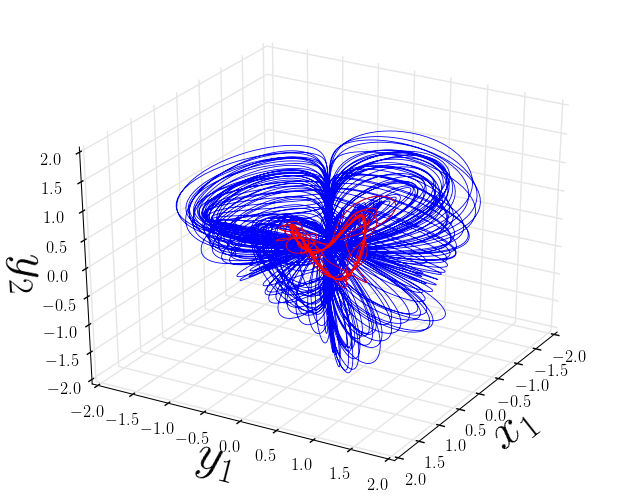
\includegraphics[width=0.35\textwidth]{Set1ssp1}
 \\
 (b) 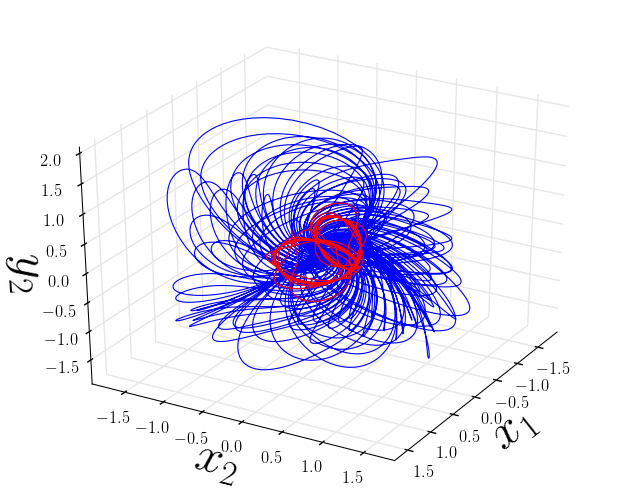
\includegraphics[width=0.35\textwidth]{Set1ssp2}
 \\
 (c) 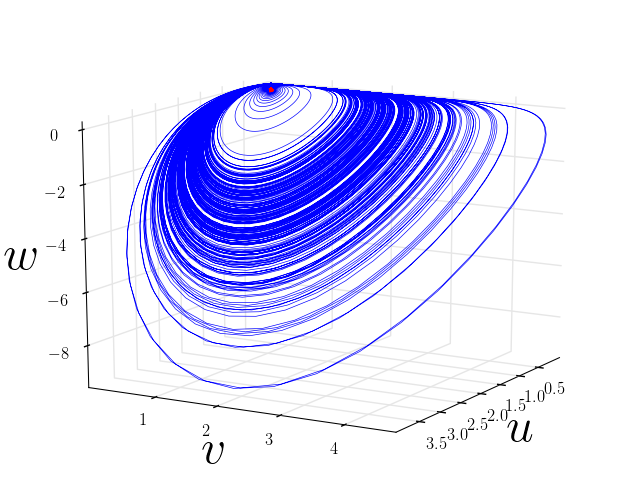
\includegraphics[width=0.35\textwidth]{Set1invpol}
 \\
 (d) 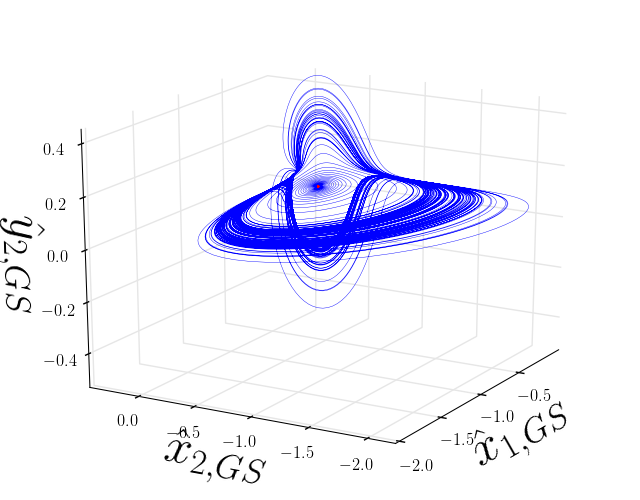
\includegraphics[width=0.35\textwidth]{Set1sspred}
\caption{\twoMode\ flow integrated for 500 time units with the initial
condition $x_0 = (0.439966, 0, 0.386267, 0.070204)$ close to the relative
equilibrium corresponding to the second root in \refeq{eq:eqvaset1}.
Projections of 4D $\SOn{2}$ equivariant \statesp\ (a, b), symmetry invariant
flow (c) and symmetry reduced flow obtained using \mslices\ (d). In each figure,
first 100 time units are drawn red. Note that in the equivariant projections (a and b)
flow traces the group orbit and then falls into the strange attractor, whereas
in the symmetry reduced representations (c and d) time orbit spirals out from
a point as one expects.
}
\label{fig:Set1}
\end{figure}

\subsection{Symbolic dynamics}

\begin{figure}%[H]
\centering
 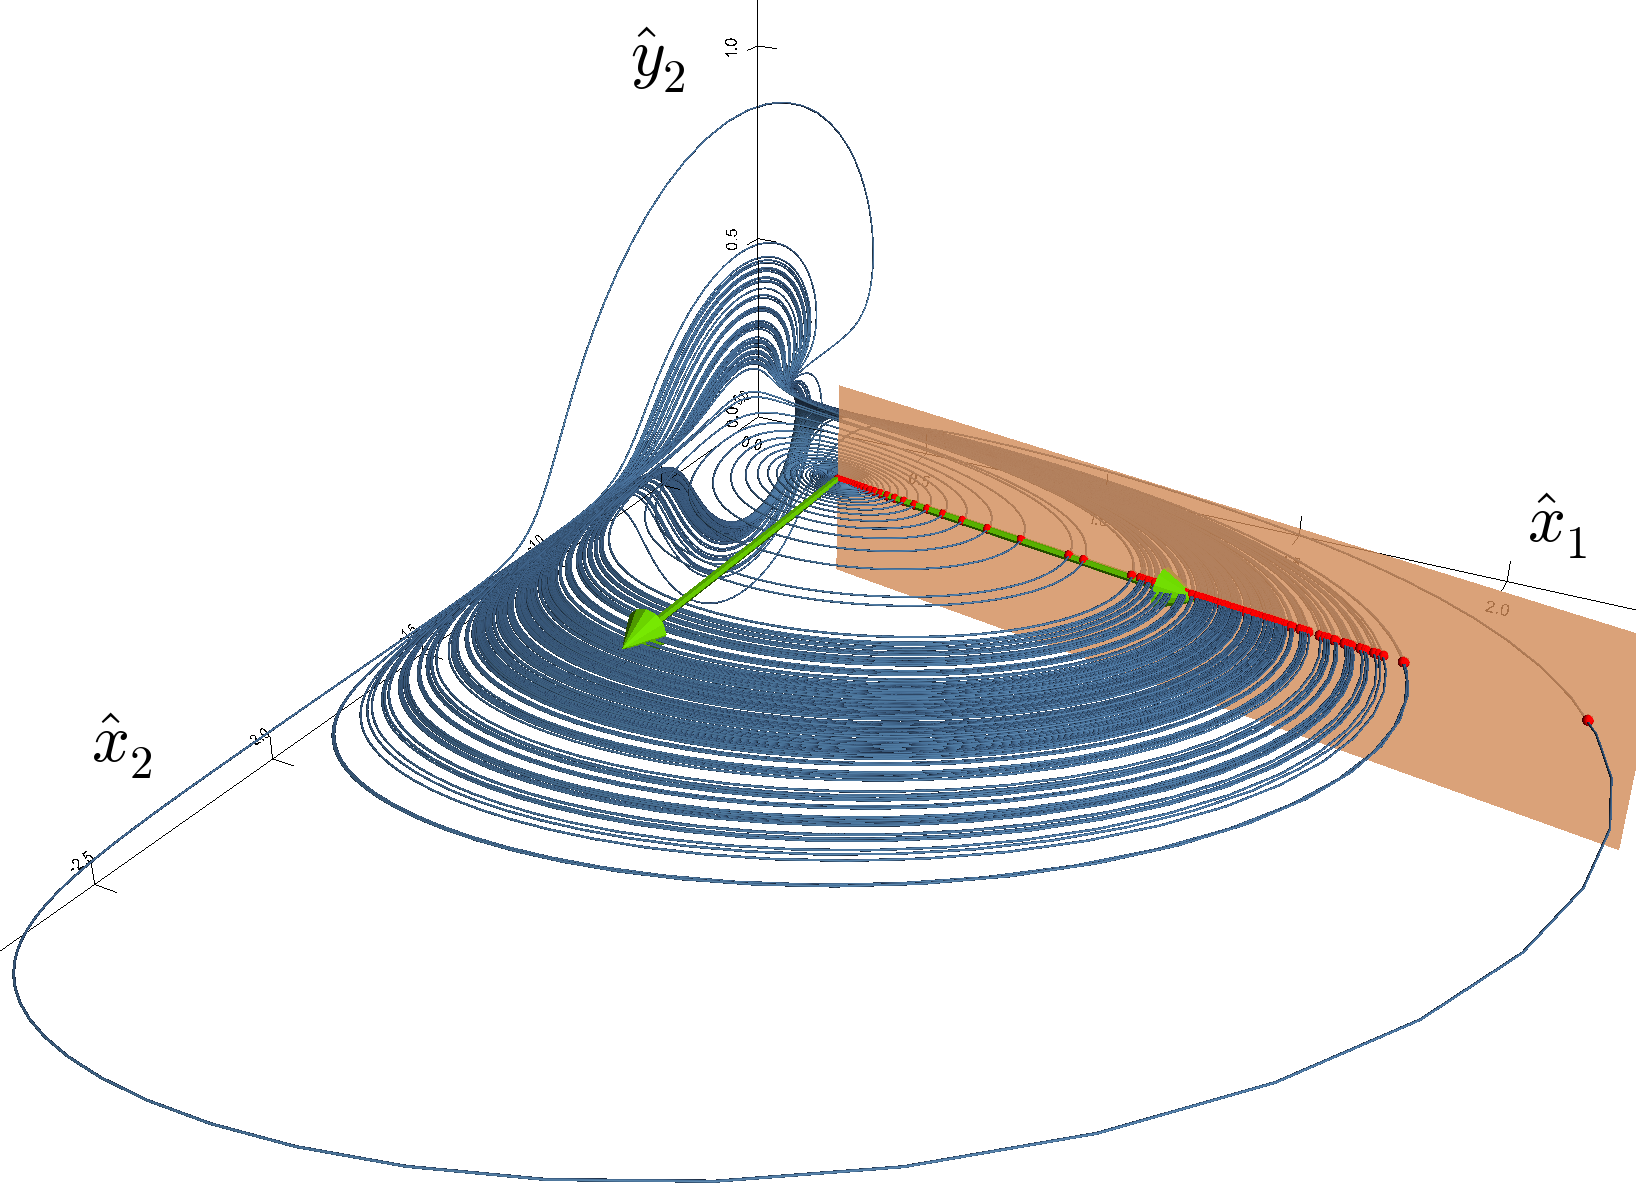
\includegraphics[width=0.45\textwidth]{BBpsecthd}
\caption{
Symmetry reduced flow within the slice hyperplane (blue). Arrows
show the unstable directions of the equilibria. Poincar\'e section, shown as
a transparent plane, involves the \reqv\ $(0.439966, 0, 0.386267, 0.070204)$
and the direction towards which the small perturbations at the \reqv\ will expand.
Intersections of the flow with the Poincar\'e section are marked with black dots.
}
\label{fig:BBpsecthd}
\end{figure}

\begin{figure}
\centering
  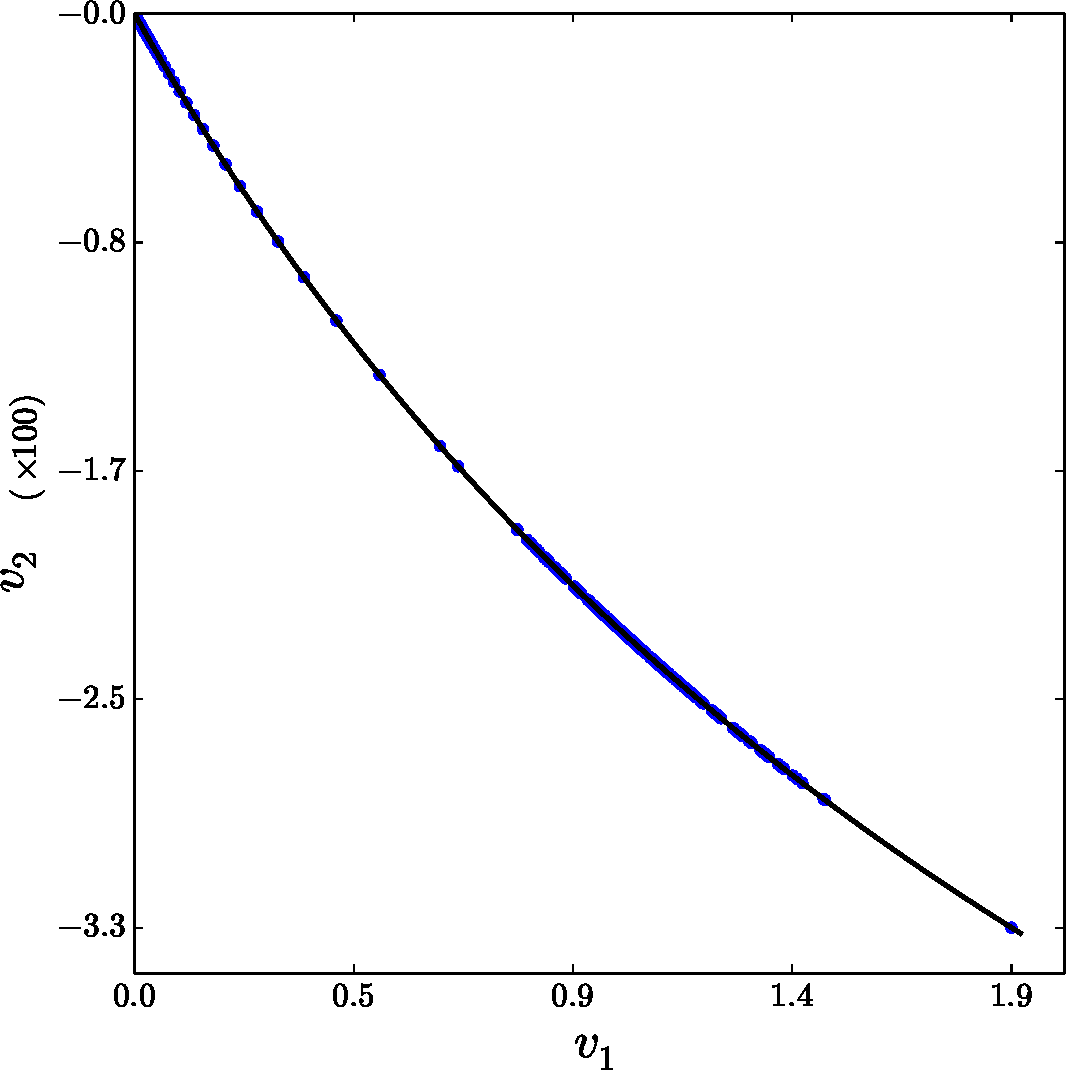
\includegraphics[width=0.23\textwidth]{BBpsectonslice}
  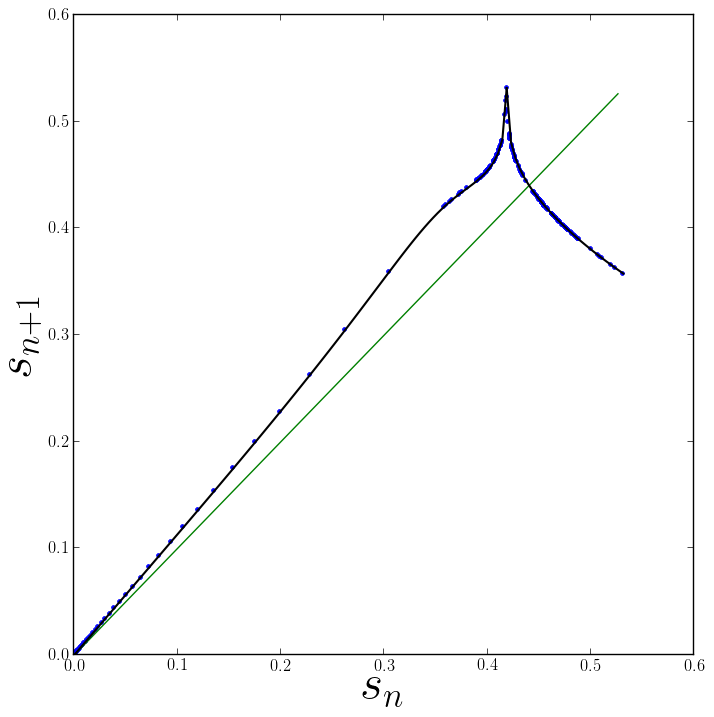
\includegraphics[width=0.22\textwidth]{BBretmaponslice}
\caption{(a) The Poincar\'e section involving the \reqv\ and its unstable direction.
		  See \reffig{fig:BBpsecthd} for its 3D visualization.
		  (b) Poincar\'e return map of arclengths along the Poincar\'e section
		  in (a).}
\label{fig:psectandretmap}
\end{figure}

%\begin{figure}%[H]
%\centering
 %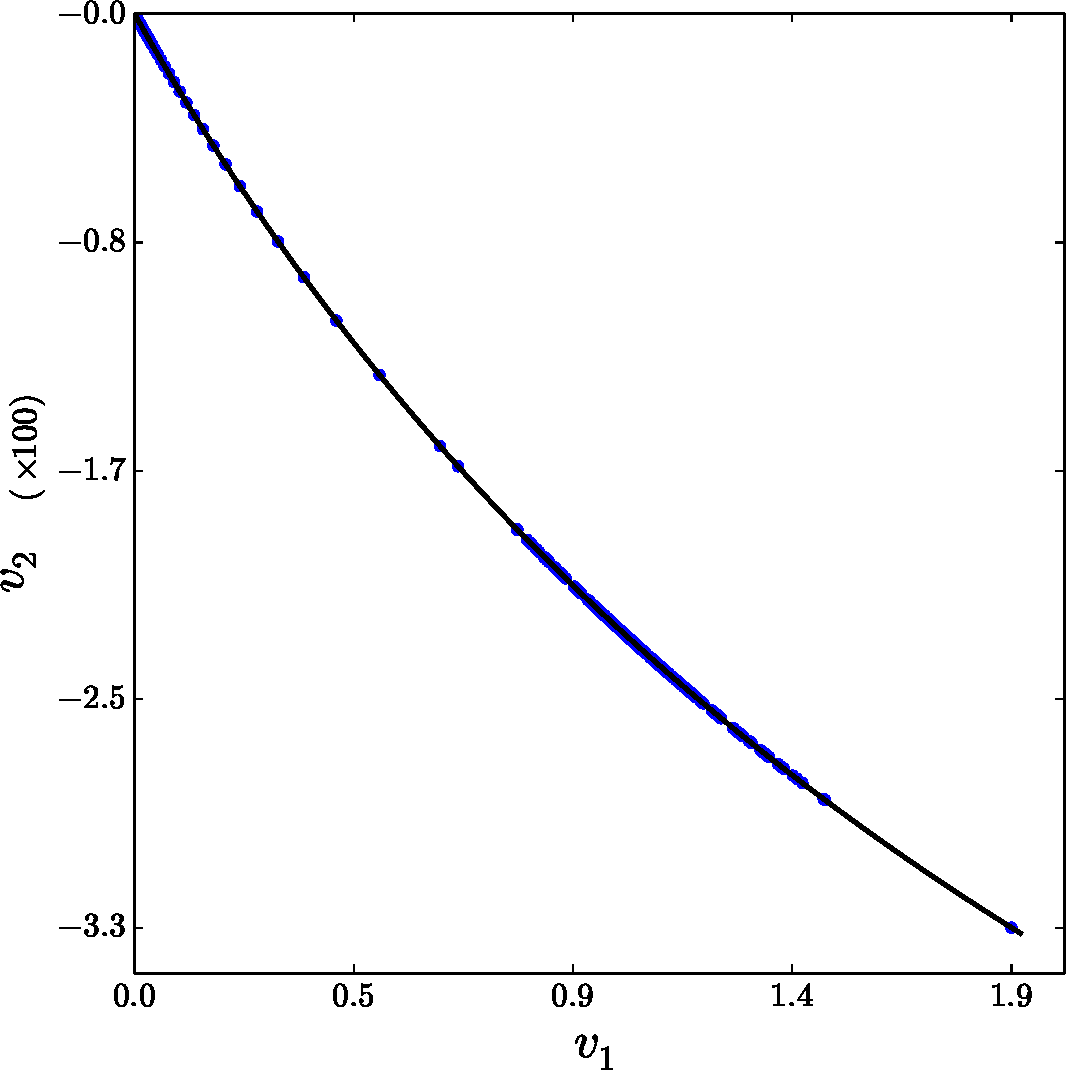
\includegraphics[width=0.45\textwidth]{BBpsectonslice}
%\caption{The Poincar\'e section involving the \reqv\ and its unstable direction.
		  %See \reffig{fig:BBpsecthd} for its 3D visualization.}
%\label{fig:BBpsectonslice}
%\end{figure}

%\begin{figure}%[H]
%\centering
 %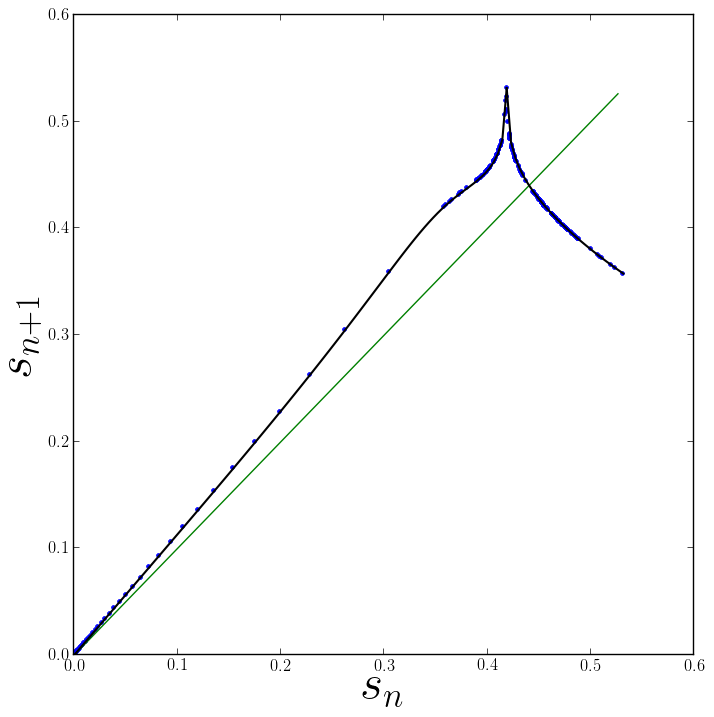
\includegraphics[width=0.45\textwidth]{BBretmaponslice}
%\caption{Poincar\'e return map of arclengths along the Poincar\'e section
		%shown in \reffig{fig:BBpsectonslice}.}
%\label{fig:BBretmaponslice}
%\end{figure}

\begin{figure}%[H]
  \begin{center}
  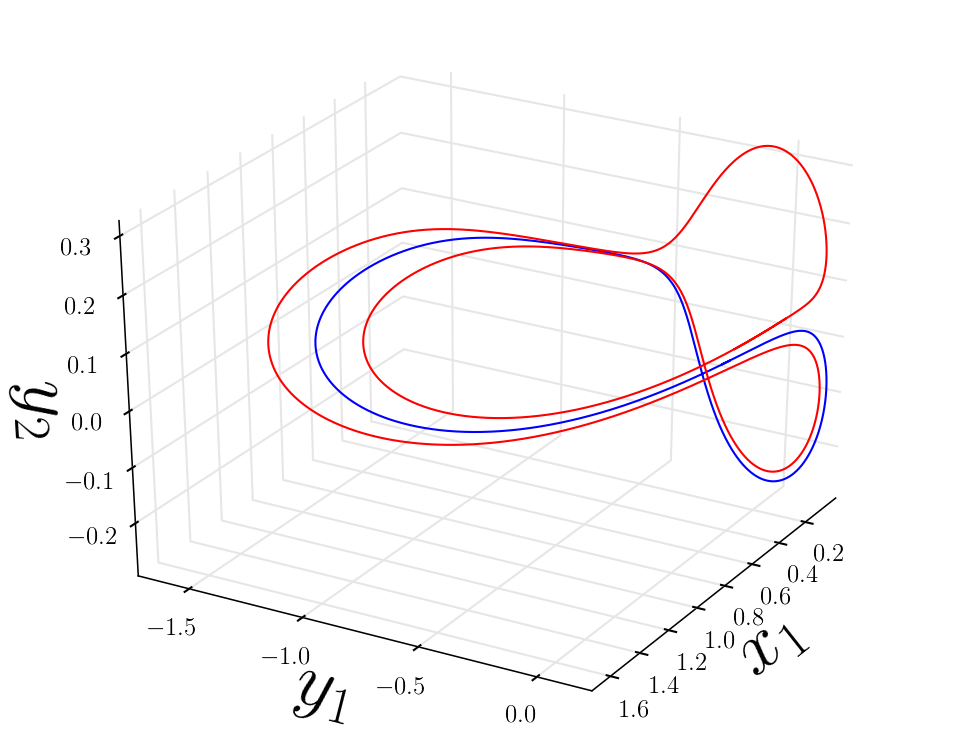
\includegraphics[width=0.45\textwidth]{BBrpo}
  \end{center}
  \caption{
	\Rpo s \cycle{1} and \cycle{01} embedded in the strange attractor
    of \reffig{fig:Set1}\,(d).
    }
  \label{fig:BBrpo1-01}
\end{figure}

\rpo s and their binary itineraries, the two shortest cycles
\cycle{1} and \cycle{01} are plotted in
\reffig{fig:BBrpo1-01}.


%SO2-equivariant equations:
%\bea
%\dot{x}_1 &=& (\mu_1 - r_1^2 + c_1 x_2)x_1 + c_1 y_1 y_2
%\continue
%\dot{y}_1 &=& (\mu_1 - r_1^2 - c_1 x_2)y_1 + c_1 x_1 y_2
%\continue
%\dot{x}_2 &=& (1 + a_2 r_1^2)x_2 + (x_1^2 - y_1^2) + y_2
%\continue
%\dot{y}_2 &=& (1 + a_2 r_1^2)y_2 + 2 x_1 y_1 - x_2
%\continue
		  %&& \mbox{where } r_1^2 = x_1^2 + y_1^2\, , \quad r_2^2 = x_2^2 + y_2^2
%\,.
%\label{2mode4Dset1}
%\eea


%%%%%%%%%%%%%%%%%%%%%%%%%%%%%%%%%%%%%%%%%%%%%%%%%%%%%%%%%%%%%%%%%%%%%%%%%%%%%%%%%%%%%%%%%%%%%%%%%%
\subsection{To do}
\label{s:ToDo}

\begin{itemize}
  \item[10.11] Visualizations of the 4-dimensional {\twoMode} system
  \item[10.1?] draw a group orbit for the {\twoMode} model
  \item[10.22] {\twoMode} system in polar coordinates (maybe skip)
  \item[10.23] The \reqva\ of the {\twoMode} system
  \item[10.24] Plotting the \reqva\ of
           the {\twoMode} system in invariant coordinates
  \item[10.25] Plotting the \reqva\ of
           the {\twoMode} system in Cartesian coordinates
           \refeq{2mode4D}
  \item[10.2?] construct a 2-chart atlas
           \reffig{fig:2ModeAtlas} for a {\twoMode} system
  \item
        compute analytically the \stabmat\ \Mvar\ in polar coordinates
  \item
        Study eigenvalues, keep playing with parameters. We would like
        -preferably- no \reqv\ to be attracting limit cycle, and several of
        the \reqva\ to be complex-pair unstable, leading to chaos, to be
        visualized and sliced in Cartesian coordinates.
  \item
        If you find a nice chaotic attractors, others can join in
        constructing an atlas for it. We just need one and only one
        example with non-trivial \chartBord s and at least 2 charts.
\end{itemize}

 [blah blah]

\begin{itemize}
  \item $\REQV{}{1} = (r_1,r_2,\psi)=(0.0516508, 1.26311,?)$ and
        $\REQV{}{2} = (0.467095,0.2146,?)$
  \item their plots in the Cartesian coordinates
  \item $\dot{\theta}$ to see how slow/fast are they. $\dot{\theta}$
        might be related to 4th eigenvalue, when you go back
        to Cartesian coordinates
  \item stability eigenvalues, eigenvectors of the \eqv\ $\EQV{0}$ at
        origin, at your parameter values - if it is stable, everything
        just might fall into it and die.
  \item plots of small perturbations of the above \eqv\ and \reqva\ in
        the Cartesian coordinates to see whether the dynamics looks
        chaotic
  \item $\REQV{}{1}$: 2 large positive eigenvalues looks scary - probably
        nothing re-visits this \reqv. A mildly unstable complex pair
        would have been sweeter. You get complex eigenvalue by Hopf-bifurcating off a
        stable orbit, typically.
  \item $\REQV{}{1}$: Does either unstable eigenvalue become a complex
        eigenvalue pair in Cartesian coordinates?
  \item $\REQV{}{2}$: contracting eigenvalues have very small imaginary
        part, so the presumably just rocket toward the \reqv, not much
        spiraling there. At least the unstable eigenvalue seems slow
        compared to all other eigenvalues.
  \item $\REQV{}{1}$: Does the unstable eigenvalue become a complex
        eigenvalue pair in Cartesian coordinates?
\end{itemize}

 [blah blah]



%%%%%%%%%%%%%%%%%%%%%%%%%%%%%%%%%%%%%%%%%%%%%%%%%
% 2011-09-09, 2012-03-30 Predrag: add BeThMovFr to
%            continuous.tex overheads, and ChaosBook
% replace A27movFrame*.* everywhere
\begin{figure}
  	\begin{center}
(a)
(b)
(c)
(d)
    \end{center}
  \caption{
  \twoMode, $d=4 \to 3$~dimensional $\{x_1,x_2,z\}$ projections:
  (a)
  The strange attractor.
  (b)
 (c)
 In contrast
 to the 1\dmn\ \poincBord s of \reffig{fig:2modeSects}, here ...
 (d)
  }
\label{fig:2ModeAtlas}
\end{figure}
%%%%%%%%%%%%%%%%%%%%%%%%%%%%%%%%%%%%%%%%%%%%%%%%%%

 [blah blah]

 [blah blah]

\section{Chart}
\label{s:slice}

 [blah blah]

One can write the equations for the flow in the \reducedsp\
$\dot{\sspRed} = \velRed(\sspRed)$ (for details see, for example,
\refref{DasBuch}) as
\bea
\velRed(\sspRed) &=& \vel(\sspRed)
     \,-\, \dot{\gSpace}(\sspRed) \, \groupTan(\sspRed)
\label{2modesEqMotMFrame}\\
\dot{\gSpace}(\sspRed) &=& \braket{\vel(\sspRed)}{\sliceTan{}}
                       /\braket{\groupTan(\sspRed)}{\sliceTan{}}
\,
\label{2modesreconstrEq}
\eea
which confines the motion to the \slice\ hyperplane. Thus, the dynamical
system $\{\pS,\map^t\}$ with continuous symmetry \Group\ is replaced by
the {\reducedsp} dynamics $\{\pSRed,\mapRed^t\}$: The velocity in the
full \statesp\ $\vel$ is the sum of $\velRed$, the velocity component in
the \slice\ hyperplane, and $\dot{\gSpace}\,\groupTan$, the velocity
component along the group tangent space. The integral of the {\em
reconstruction equation} for $\dot{\gSpace}$ keeps track of the group
shift in the full \statesp.


 [blah blah]


\section{Conclusions}
\label{s:concl}

 [blah blah]
Whether our method can reduce
the \SOn{2}-symmetry also for $N$-Fourier modes truncations of PDEs such as
the Kuramoto-Sivashinsky, pipe flows, etc., as long as the amplitude of
the first Fourier mode is non-zero.


\begin{acknowledgments}
We acknowledge stimulating discussion with Al Shapere.
This report addresses the questions asked in
the 2012 ChaosBook.org class.
We are indebted to Keith M. Carroll, Sarah Flynn,
Bryce Robbins,
%    \PC{Is Bryce a co-author or somebody we acknowledge?
%    Nov 16 2013 Burak talked to him: dropped out}
and
Lei Zhang
for many inspiring discussions and cross-checks of the model.
% and Edgar Knobloch for [...].
\end{acknowledgments}


\bibliography{../bibtex/siminos}
%   \fi % 2012-08-06 end of temporary \onecolumngrid


\ifdraft
    \onecolumngrid

    \newpage
\input flotsam
    \newpage
    \section{{\twoMode} simulations blog}
    \label{chap:Mathematica}
\input ../blog/Mathematica

    \newpage
    \section{{\twoMode} daily blog}
    \label{chap:2modes}
\input ../blog/2modes
    \newpage
    \section{Burak' s {\twoMode}}
    \label{chap:2modesBB}
\input ../blog/2modesBB % Predrag 2013-0810 Burak, git version only

\addcontentsline{toc}{section}{last blog entry}

%\vfill
%\begin{quote}
%{\color{red} \large
%May 1 2012,  11:30am - 2:20pm term projects due, Predrag's office
%}
%\end{quote}

\fi

\end{document}
